\section{Additive Effect Sites}

This assay is designed to detect sites witth small-effect fitness contributions.
Although knockout effects of individual sites do not reach the threshold for detectability, knocking out several may.
This assay assumes a preliminary set of single-site knockouts that exclude sites with individually-detectable fitness effects from further consideration.
Then, sets of remaining sites are sampled and knocked outt together.

In the presence of small-effect sites, a classic dose-response curve will occur as sampled set size is increased.
That is, detectable fitness effects will be observed more frequently for larger knockout sets.
The shape of this dose curve will depend on both the abundance of small-effect sites and their mean effect size.
Fitting a negative binomial distribution to the curve allows these factors to estimated.
This distribution models, for coin flips with success probability $p$, the number of successive trials required to achieve $n$ successes.
If we consider resolution of sampled sites to small-effect versus true-neutral categories as a coin flip event, then the proportion of small-effect sites will correspond to $p$ and $n$, the number of required small-effect sites to reach detctability, will be inverse to the mean effect size.
Under this framming, the dose response curve corresponds to the cumulative disribution function of an underlying negative binomial distribution.

For initial experimentts exploring this approach, we generated sammple genomes with 1,000 sites, 50 of which were designated to be small-effect siters.
Effect sizes for these sites were uniformly between 0 and 0.2, relative to the detectability threshold of 1.0.
To decide dose levels for the main assay, we first sampled 250 doses spread evenly from 1 to 1,000 sites and tested for detectable fitness effects for one sample at each dose level.
We used the interval between the lowest dose with a detected fitness effect and the highest dose without a detected fitness effect as the dosing range for the main assay, choosing five dosing levels spaced evenly across this range.
For example, in one replicate, our selected dose levels were 87, 136, 186, 236, and 286 sites.
We then performed 1,000 knockouts of site sets sampled at each level.
Among 10 replicate assays, estimates of the true site countt ranged from TODO to TODO, with a mean estimate of TODO.

\section{Epistatic Effect Sites}

\begin{figure}
  \centering
  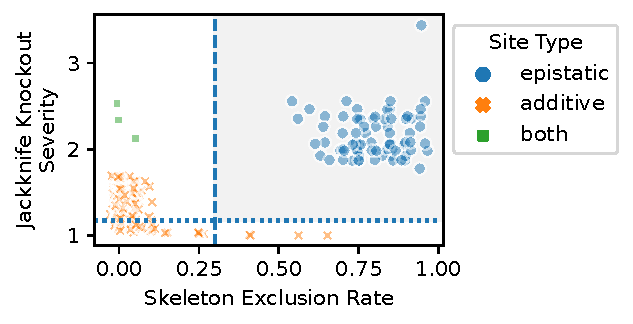
\includegraphics[width=\linewidth]{binder/teeplots/hue=site-type+style=site-type+viz=scatterplot-rect+x=skeleton-exclusion-rate+y=jackknife-knockout-severity+ext=}
  \vspace{-0.25in}
  \caption{%
    Use of knockout effect sizes and inclusion rates within ``skeletonized'' minimal viable genomes to distinguished small-effect and epistatic genome sites.
  }
  \label{fig:epistatic}
  \vspace{-0.25in}
\end{figure}


This assay uses minimal viable genomes, ``skeletons,'' as the basis for estimation.
Repeated stochastic successive knockout process until no more sites can be removed to generate a sample of skeletons.
The intuition is that sites that appear infrequently in skeletons but not others are epistatic.
However, additive small-effect sites will also appear sometimes appear outside skeletons.

We can use knockout effect size to differentiate these cases.
For this procedure, we iterate through the skeleton and do ``jackknife'' single site knockouts.
If the marginal knockout effect size of this site is very small, then it is probably an additive site.
If the marginal knockout effect of the site in the skeleton context is big, it is probably an epistatic effect site --- with the rest of its redundant sites already excluded from the skeleton.
Figure \ref{fig:epistatic} shows this distinction.

% Create Sample Genome
% Create a genome with 4,000 distinct sites.

% Let 5% of sites have an additive knockout fitness effect below detectability threshold (uniform between 0 and 0.7 fitness effect).

% Assign 20 sets of epistatic effects, with 5 sites per set. Apply a set-specific fitness penalty between 0.7 and 1.6 when all sites in a set are knocked out.

% Fitness 1.0 is considered the threshold for detectability

% neutral      3706
% additive      195
% epistasis      94
% both            5

% "Skeletons" are minimal sets of genome sites that maintain wile-type fitness. Skeletons can be generated by sequentially removing sites from the genome, until no further sites can be removed without detectably reducing fitness.

% Sample 20 skeletons.

% "Skeletons" are minimal sets of genome sites that maintain wile-type fitness. Skeletons can be generated by sequentially removing sites from the genome, until no further sites can be removed without detectably reducing fitness.

% Sample 20 skeletons.

% Use Skeleton Jackknifes to Differentiate Epistasis versus Additive Sites
% Our goal is to isolate epistatic sites and then count them up.

% Do this by setting thresholds for skeleton exclusion frequency and jackknife knockout severity, then counting sites that exceed both thresholds.

% First, set the skeleton exclusion frequency threshold at 0.3. Then, look at all points excluded less than 30% of the time. Take the 20th percentile of these sites' jackknife knockout severities. This is the jackknife knockout severity threshold.

% Then, count sites that exceed both thresholds.

% est = assay_epistasis_naive(
%     df_skeletons,
%     exclusion_frequency_thresh=0.3,
%     jackknife_severity_thresh=0.2,
% )
% est
% {'num epistasis sites estimate': 80,
%  'exclusion frequency cutoff': 0.3,
%  'jackknife severity cutoff': 1.1739066427089908}
% For comparison, the actual count of epistasis sites is

% df_genome["site type"].value_counts()["epistasis"]
% 94
% This estimate could probably be improved with mark-recapture methods as used in the "agnostic" methods.

% Note the presence of very small-effect additive sites (i.e., low jackknife knockout severity) with high exclusion rates. This is why we need jackknife severity to identify epistatic sites.

\section{Any Effect Sites}

Skeletons can be put to another use to try to directly estimate the number of sites that have any fitness effect.
Reframed, skeletoniz.
Any site that has a fitness benefit should, in principle, potentially appear within a skeleton.
Skeletons randomly sample from among these sites.
Framed this way, sampling a skeleton genome is not unlike a trap sampling study used by wildlife biologists.
Extensive, well-developed mathematics exists around this problem.
Such math will need to be careful to account for ``shyness'' --- uneven probability for some sites appearing in a skeleton.
We propose to use the Burnham-Overton estimation procedure.
We give it a distribution of, among the sites that appeared within skeletons, the number of skeletons they appeared in and it gives us a total population estimate

% # Burnham, Kenneth P., and W. Scott Overton.
% # "Robust estimation of population size when capture probabilities vary among
% # animals." Ecology 60.5 (1979): 927-936.
% # https://doi.org/10.2307/1936861

% Create Sample Genome
% Create a genome with 10,000 distinct sites.

% Let 4% of sites have a knockout fitness effect below detectability threshold. Effect sizes are distributed uniformly between 0 and 0.7, relative to the detectability threshold of 1.0.

% Add 40 epistatic sets, each with 4 sites. Fitness consequences of magnitudes between 0.7 and 1.6 occur when all sites within an epistatic set are knocked out.

% Overlap is allowed --- n individual sites may have both additive and epistatic effects.

% num_sites = 10000
% distn = lambda x: np.random.rand(x) * 0.7
% additive_array = create_additive_array(num_sites, 0.04, distn)
% epistasis_matrix = create_epistasis_matrix_disjoint(num_sites, 40, 4)
% genome = GenomeExplicit(
%     [
%         CalcKnockoutEffectsAdditive(additive_array),
%         CalcKnockoutEffectsEpistasis(epistasis_matrix, effect_size=(0.7, 1.6)),
%     ],
% )

% neutral      9445
% additive      395
% epistasis     155
% both            5
% Name: site type, dtype: int64

% How many functional (i.e., non-neutral) sites are there?

% num_functional_sites = (df_genome["site type"] != "neutral").sum()
% num_functional_sites
% 555
% Perform Skeletonizations
% "Skeletons" are minimal sets of genome sites that maintain wile-type fitness. Skeletons can be generated by sequentially removing sites from the genome, until no further sites can be removed without detectably reducing fitness.

% How many unique sites show up in any skeleton? (i.e., num sites with direct evidence of functionality)

% np.any(
%     (~skeletons.astype(bool)),
%     axis=0,
% ).sum()
% 504
% Estimate Number Functional Sites
% The skeletonization process can actually be interpreted as a mark-recapture experiment. Just like field researchers counting rabbits, we can estimate the total population of functional sites from the rate at which we "re-capture" specimens. (Here, "re-capture" means that a site is included in more than one skeleton.)

% Note that statistics taking into account bias in capture probability (aka "trap shyness") are necessary. This implementation uses a nonparametric jackknife estimator due to Burnham and Overton (see source code for details).

% assay_agnostic_naive(df_skeletons)
% {'num sites estimate': 558.3499999999999,
%  'num sites 95% CI': (533.2059805122569, 583.4940194877429)}
% For comparison the actual number of functional sites is

% num_functional_sites
% 555
